\documentclass[11pt]{article}
\usepackage{colacl}
\usepackage{float}
\usepackage{graphicx}
\usepackage[T1]{fontenc}
\usepackage[utf8]{inputenc}
\usepackage{listings}
\usepackage{amssymb}
\usepackage{amsmath}
\usepackage{bm}
\graphicspath{{img/}}
\DeclareUnicodeCharacter{F8FF}{$\diamond$}
\sloppy

\title{COMP30027 Assignment 2: Report}
\author
{Anonymous}



\begin{document}
\maketitle

\section{Introduction}\label{sec:intro}
% Introduction: a short description of the problem and data set

Sentiment analysis focuses on the classifying text into sentiments.
My goal is to apply sentiment analysis to develop and train three reliable sentiment classifiers and one baseline for {T}witter posts (tweets).
This involves extracting and selecting useful features from a dataset of tweets, 
then choosing and evaluating highly reliable classifiers.

\subsection{Dataset}\label{sec:dataset}

The dataset provided contains two lists of tweets/instances made prior to 2017 \cite{dataset}.
The training set in \texttt{Train.csv} contains $21802$ labelled instances and the testing set in \texttt{Test.csv} contains $6099$ unlabelled instances. 
For each instance, included is the text and tweet ID. 
The tweets included vary in content.
For example, some are not in English: ``\textit{season in the sun versi nirvana rancak gak..slow rockkk...}''.
Tweets can either be "positive", "neutral" or "negative", distributed as shown in Figure~\ref{fig:sent-dist}.

\begin{figure}[H]
	\centering
	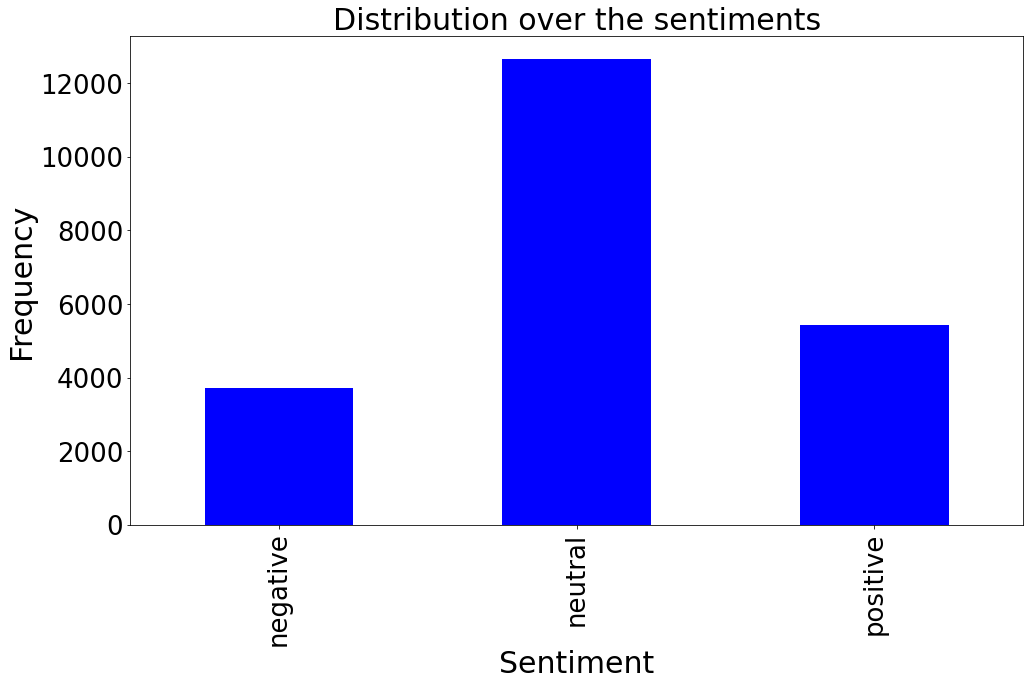
\includegraphics[width = 0.45\textwidth]{sentiment-distribution.png}
	\caption{Training sentiment distribution}
	\label{fig:sent-dist}
\end{figure} 

\section{Methodology}
% Method: Introduce the used feature(s), and the rationale behind including them. Explain the classifiers
% and evaluation method(s) and metric(s) you have used (and why you have used them). This should be
% at a conceptual level; a detailed description of the code is not appropriate for the report. The description
% should be similar to what you would see in a machine learning conference paper.

The following methods are developed with reference to prior works on {T}witter sentiment analysis \cite{go09,nltk,robustnoisy10}.

\subsection{Instance cleaning}

Some features extracted rely on the text in the tweets being cleaned.
Cleaning involves removing stopwords (Section~\ref{sec:stopwords}), links, hashtags, mentions, numbers, non-alphanumeric characters.
Also performed is the reduction of repeated letters with more than two occurrences, as suggested by Go et al. \shortcite{go09}.

\subsubsection{Stopwords}\label{sec:stopwords}

Manual stopword list construction is tedious and inexhaustive (consider other languages). 
Instead, I start with the {P}ython Natural Language Toolkit's (\texttt{NLTK}) stopword list, which includes non-English languages \cite{nltk}.

\begin{figure}[H]
	\centering
	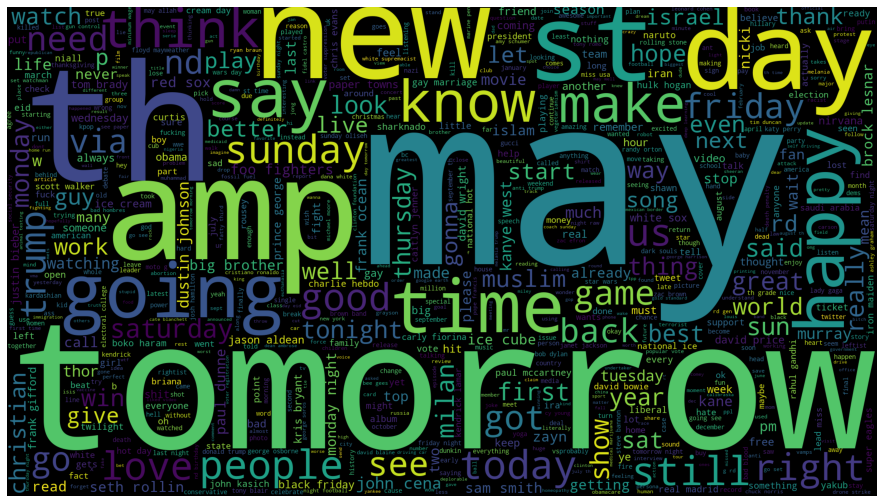
\includegraphics[width = 0.4\textwidth]{wc/all-clean-nltk.png}
	\caption{Word cloud with \texttt{NLTK} stopword removal}
	\label{fig:wc-nltk}
\end{figure}

Next, based on Figure~\ref{fig:wc-nltk}, some extra words are manually added to the list, leading to the final vocabulary list in Figure~\ref{fig:wc-final}.

\begin{figure}[H]
	\centering
	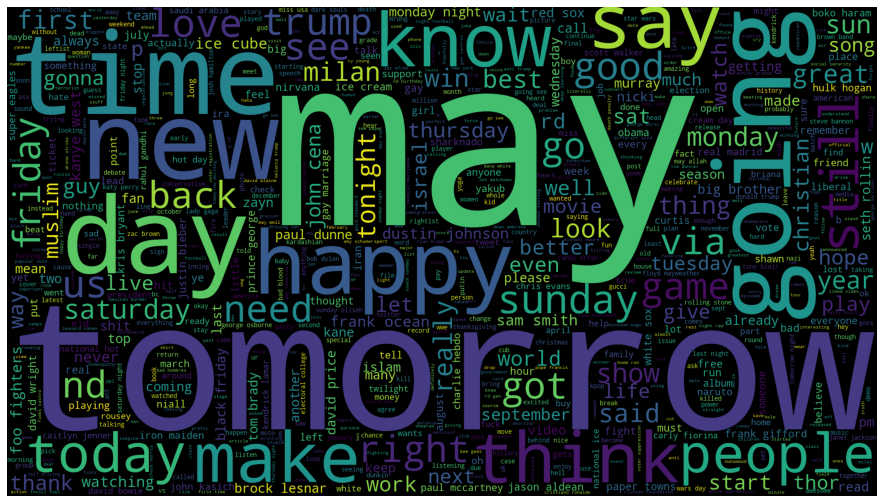
\includegraphics[width = 0.4\textwidth]{wc/all-clean-final.png}
	\caption{Word cloud with modified \texttt{NLTK} stopword removal}
	\label{fig:wc-final}
\end{figure} 

\subsection{Feature extraction}

These features are all chosen for their potential correlations with sentiments.

\subsubsection{{T}witter features}

First, I extract platform-specific features from the tweets: 
hashtags, mentions, and links \cite{go09,robustnoisy10}.
These are integrated within the platform, meaning they are widely used (commonplace in tweets).

\subsubsection{Linguistic features}

Next, linguistic features are extracted and used to tokenize the tweet in different ways: 
part-of-speech tags, lemmas, lemma 2-grams, phonetics (phenomes of words), punctuation, and emoticons \cite{robustnoisy10,nltk,cmudict}.
Lemmas are preferred over words, as they group words of the same root \cite{nltk}.


Emoticons are identified as string combinations of eye, middle and mouth characters,
a different method to Go et al. \shortcite{go09},
since they misses emoticons, such as the crying \texttt{:'(}.
Emoticons are then categorized into happy \texttt{:)}, sad \texttt{:(}, neutral \texttt{:|} or surprised \texttt{:o}.

\subsubsection{Metric features}

These are numeric counts of feature types within a tweet: words, characters, alphabetic characters, links, hashtags, mentions, and emoticons.
Also considered are average word length and if a tweet is quoting another.

\subsubsection{How many features per feature type is enough?}

With over 20000 instances in the training dataset, some feature types generate a numerous unique results.
Minimizing the feature space with a limit of features per feature type reduces model complexity.
To determine this number $M_f$, the top candidate classifiers are compared for each of $M_f \in \lbrace 10, 100, 1000, 5000 \rbrace$ by the accuracies found using Section~\ref{sec:choosing2}.

\subsubsection{Vectorization}

At the time that the data was collected, tweets were limited to 140 characters \cite{tweetlen}.
This means that features appear once (at most twice) in a tweet.
Therefore, non-metric features are vectorized by occurrence counts, 
as TF-IDF is not applicable with near-binary features. 

\subsection{Classifier Selection}

\subsubsection{Baseline}

The baseline model used is the 0-R: most frequent class (Classifier 4).
The three chosen models (Classifiers 1, 2, and 3) need to outperform this.

\subsubsection{Classifier Candidates}\label{sec:allcandidates}

The following classifier/parameter combinations are considered for the final three models. 

\textbf{Multinomial/Bernoulli Naive Bayes}:
\begin{table}[h]
	\begin{center}
		\begin{tabular}{|c|c|}			
			\hline
			Parameter & Options \\
			\hline
			Include Priors & Yes, No \\
			$\alpha$ Smoothing & 0, 1, 10 \\
			\hline
		\end{tabular}
		\caption{Naive Bayes Parameters}
		\label{tbl:nb-options}
	\end{center}
\end{table}

\textbf{Logistic Regressions}:
\begin{table}[h]
	\begin{center}
		\begin{tabular}{|c|c|}			
			\hline
			Parameter & Options \\
			\hline
			Fit Intercept & Yes, No \\
			Maximum Iterations & 100, 500 \\
			Optimization & \texttt{sag}, \texttt{saga} \\
			\hline
		\end{tabular}
		\caption{Logistic Regression Parameters}
		\label{tbl:lr-options}
	\end{center}
\end{table}

\textbf{Decision Trees}:
\begin{table}[h]
	\begin{center}
		\begin{tabular}{|c|c|}			
			\hline
			Parameter & Options \\
			\hline
			Maximum Depth & 1, 100, 500 \\
			\hline
		\end{tabular}
		\caption{Decision Tree Parameters}
		\label{tbl:dt-options}
	\end{center}
\end{table}

\textbf{$K$ Nearest Neighbours}:
\begin{table}[H]
	\begin{center}
		\begin{tabular}{|c|c|}			
			\hline
			Parameter & Options \\
			\hline
			$K$ & 1, 10, 100, 500 \\
			Vote Weighting & \texttt{uniform}, \texttt{distance} \\
			\hline
		\end{tabular}
		\caption{K-Nearest Neighbour Parameters}
		\label{tbl:knn-options}
	\end{center}
\end{table}

\textbf{Support Vector Classifiers}:
\begin{table}[H]
	\begin{center}
		\begin{tabular}{|c|c|}			
			\hline
			Parameter & Options \\
			\hline
			Kernel & Linear, Cubic \\
			Regularization $C$ & 0.1, 1, 3 \\
			Decision Function & One-v-One, One-v-Rest \\
			\hline
		\end{tabular}
		\caption{Support Vector Classifier Parameters}
		\label{tbl:svc-options}
	\end{center}
\end{table}


\subsection{Evaluation}\label{sec:evaluations}

\subsubsection{Which Parameter Configurations Are Best?}\label{sec:choosing2}

Of the combinations in Section~\ref{sec:allcandidates}, 
the top three (Classifiers 1, 2, and 3) are determined with the following scoring system.
First, cross-validation scores are calculated on the training set.
Next, cross-validation is performed on the maximum subset of data with a uniform sentiment distribution.
The 10 scores are averaged $\bar{x}$, and their standard deviation $s$ found. 
The best candidate configurations have the highest bound for the right-sided $95\%$ confidence interval of mean cross-validation scores:
\begin{align*}
	\text{95\% C.I. Bound} &= \bar{x} - \mathbb{F}_{t}^{-1}(0.95) \times \frac{s}{\sqrt{n}} \\
	&= \bar{x} - 1.8331 \times \frac{s}{\sqrt{10}}
\end{align*}
where $t$ is the $t$-distribution with $df = 9$ and $n = 10$.

\subsubsection{Evaluation Metrics}\label{sec:evalmetrics}

Accuracies, precisions, recalls and $F_1$ scores (per sentiment) are generated for each classifier that makes it past Section~\ref{sec:choosing2}.

\subsubsection{Which models are label distribution agnostic?}

It is unknown whether the \texttt{Test.csv} and \texttt{Train.csv} sentiments are similarly distributed, 
so evaluation metrics from Section~\ref{sec:evalmetrics} are calculated for four $4:1$ train/test splits.
Evaluation metrics are generated on the combinations in Table~\ref{tbl:train-test} of these training and testing splits.
The metrics are then compared to determine which models are agnostic to sentiment distributions.

\begin{table}[H]
	\begin{center}
		\begin{tabular}{|l|l|}			
			\hline
			Training & Testing \\
			\hline
			Uniform & Uniform \\
			Given & Given \\
			Given & Uniform \\
			Uniform & Given \\
			\hline
		\end{tabular}
		\caption{Training and testing splits}
		\label{tbl:train-test}
	\end{center}
\end{table}

Where ``Given'' denotes a set of data with sentiment distributions similar to those in Figure~\ref{fig:sent-dist},
and ``Uniform'' denotes a maximum subset of data with uniformally distributed sentiments.

\section{Results}\label{sec:results}
% Results: Present the results, in terms of evaluation metric(s) and, ideally, illustrative examples and diagrams.

\subsection{Highest cross-validation accuracy per number of maximum features}\label{sec:mfresults}

After generating classifiers for each of the $M_f$ values, 
the following boasted the highest scores calculated in Section~\ref{sec:choosing2}.

\begin{table}[H]
	\begin{center}
		\begin{tabular}{|l|l|}			
			\hline
			Parameter & Value \\
			\hline
			Classifier & Logistic Regression \\
			Fit Intercept & No \\
			Maximum Iterations & 500 \\
			Optimization & \texttt{sag} \\
			\hline\hline
			$\bar{x}$ &  0.5491\\
			$s$ &  0.05083 \\
			95\% C.I. Bound & 0.5196 \\
			\hline
		\end{tabular}
		\caption{$M_f = 10$ Top classifier}
		\label{tbl:mf10}
	\end{center}
\end{table}

\begin{table}[H]
	\begin{center}
		\begin{tabular}{|l|l|}			
			\hline
			Parameter & Value \\
			\hline
			Classifier & Logistic Regression \\
			Fit Intercept & Yes \\
			Maximum Iterations & 500 \\
			Optimization & \texttt{sag} \\
			\hline\hline
			$\bar{x}$ &  0.5852\\
			$s$ &  0.03187 \\
			95\% C.I. Bound & 0.5667 \\
			\hline
		\end{tabular}
		\caption{$M_f = 100$ Top classifier}
		\label{tbl:mf100}
	\end{center}
\end{table}

\begin{table}[H]
	\begin{center}
		\begin{tabular}{|l|l|}			
			\hline
			Parameter & Value \\
			\hline
			Classifier & Bernoulli N.B. \\
			Include Priors & Yes \\
			$\alpha$ Smoothing & 5 \\
			\hline\hline
			$\bar{x}$ &  0.6179\\
			$s$ &  0.01537 \\
			95\% C.I. Bound & 0.6090 \\
			\hline
		\end{tabular}
		\caption{$M_f = 1000$ Top classifier}
		\label{tbl:mf1000}
	\end{center}
\end{table}


\begin{table}[H]
	\begin{center}
		\begin{tabular}{|l|l|}			
			\hline
			Parameter & Value \\
			\hline
			Classifier & Bernoulli N.B. \\
			Include Priors & Yes \\
			$\alpha$ Smoothing & 1 \\
			\hline\hline
			$\bar{x}$ &  0.6372\\
			$s$ & 0.01438 \\
			95\% C.I. Bound & 0.6288 \\
			\hline
		\end{tabular}
		\caption{$M_f = 5000$ Top classifier}
		\label{tbl:mf5000}
	\end{center}
\end{table}

\begin{table}[H]
	\begin{center}
		\begin{tabular}{|l|l|}			
			\hline
			Parameter & Value \\
			\hline
			Classifier & Bernoulli N.B. \\
			Include Priors & Yes \\
			$\alpha$ Smoothing & 1 \\
			\hline\hline
			$\bar{x}$ &  0.6361\\
			$s$ & 0.01028 \\
			95\% C.I. Bound & 0.6301 \\
			\hline
		\end{tabular}
		\caption{$M_f = 10000$ Top classifier}
		\label{tbl:mf10000}
	\end{center}
\end{table}

It appears that $\emph{accuracy} \varpropto M_f$.
The final classifer models are trained with $M_f = 10000$ to maximize accuracy.

\subsection{Top 3 parameter/classifier configurations for $M_f = 10000$}\label{sec:top3}

The following classifiers have the highest scores calculated in Section~\ref{sec:choosing2}:

\begin{table}[H]
	\begin{center}
		\begin{tabular}{|l|l|}			
			\hline
			Parameter & Value \\
			\hline
			Classifier & Bernoulli N.B. \\
			Include Priors & Yes \\
			$\alpha$ Smoothing & 1 \\
			\hline\hline
			$\bar{x}$ &  0.6361\\
			$s$ & 0.01028 \\
			95\% C.I. Bound & 0.6301 \\
			\hline
		\end{tabular}
		\caption{Classifier 1}
		\label{tbl:1st10000}
	\end{center}
\end{table}

\begin{table}[H]
	\begin{center}
		\begin{tabular}{|l|l|}			
			\hline
			Parameter & Value \\
			\hline
			Classifier & Bernoulli N.B. \\
			Include Priors & No \\
			$\alpha$ Smoothing & 1 \\
			\hline\hline
			$\bar{x}$ &  0.6365\\
			$s$ &   0.01159 \\
			95\% C.I. Bound & 0.6298 \\
			\hline
		\end{tabular}
		\caption{Classifier 2}
		\label{tbl:2nd10000}
	\end{center}
\end{table}

\begin{table}[H]
	\begin{center}
		\begin{tabular}{|l|l|}			
			\hline
			Parameter & Value \\
			\hline
			Classifier & Multinomial N.B. \\
			Include Priors & Yes \\
			$\alpha$ Smoothing & 1 \\
			\hline\hline
			$\bar{x}$ &  0.6343\\
			$s$ &   0.01428 \\
			95\% C.I. Bound & 0.6260 \\
			\hline
		\end{tabular}
		\caption{Classifier 3}
		\label{tbl:3rd10000}
	\end{center}
\end{table}

\subsection{Evaluation metrics for the final 4 models}

Generated based on Section~\ref{sec:evalmetrics}. 
Per-class metrics are shown in order of postive (+), neutral (n), then negative (--) sentiments.
See Section~\ref{sec:appa} (Appendix).

\section{Analysis}
% Discussion / Critical Analysis: Contextualise the systems' behaviour, based on the understanding of the
% subject materials (This is the most important part of the task in this assignment).

% Contextualise implies that we are more interested in seeing evidence of you have thought about the task
% and determining reasons for the relative performance of different methods, rather than the raw scores of
% the different methods you selected. This is not to say that you should ignore the relative performance of
% different runs over the data, but rather that you should think beyond simple numbers to the reasons that
% underlie them.

\subsection{How $M_f$ modifies the models}\label{sec:mfanalysis}
The results from Section~\ref{sec:mfresults} highlight a pattern.
For lower max feature values $M_f$, the top models are logistic regressions,
whereas for $M_f \geq 1000$, the best are bernoulli naive Bayes. 
This suggests that logistic regressions are more versatile with smaller dimensions of features than other classifiers.
This is likely due to their optimization feature weights.
A smaller feature space results in fewer possible local minima.
With fewer local minima, it is likely that the true error rate minimum is found with the feature weights.


For $M_f \geq 1000$, the bernoulli naive Bayes models have the highest bound for the right-sided 95\% cross-validation scores with larger feature spaces.
Most of the classifiers considered rely on solving an optimization problem to determine a support vector, or a set of weights.
The naive Bayes models do rely on optimization, and are therefore more reliable with large feature spaces.

\subsection{The best classifier/parameter configurations}

The best classifier configurations with a large feature space are naive Bayes estimators, as shown in Section~\ref{sec:top3}.
The highest scoring model is the bernoulli naive Bayes, with $\alpha = 1$ laplace smoothing and sentiment label priors included.


The Classifiers 1, 2, and 3 all perform better than the baseline model. 
The only exception is in the recalls of the 0-R, which the baseline model has the best results for.
However, this is misleading since the 0-R baseline classifier labels all instances with the same class, 
guarranteeing that one of the classes has no false negative values.


With the used feature set, bernoulli naive Bayes classifiers are more applicable, since most features only appear in a tweet as binary events.
This is reflected in the best possible model, while the multinomial model is still high accuracy relative to non-naive Bayes methods (Table~\ref{tbl:3rd10000}).

\pagebreak
The naive Bayes classifiers yield higher accuracies than the other considered classifiers, since they scale easily with the size of the feature space (see Section~\ref{sec:mfanalysis}).
To improve the accuracy of optimization-reliant classifiers, I would need to either start with an initial state (of weights or support vectors) that is known to be near the true error maximum, 
or to train the models multiple times with a large number of iterations.
Both of these options cannot be achieved with limited time, and with a large feature space as I am using.


The top models rely on laplace smoothing with $\alpha = 1$, implying that there is a need to account for potentially missing values.
However, as the $alpha$ for the smoothing increases further, 
the features present in the data are undermined in predictions, and the resulting models are less accurate. 

\subsection{The most sentiment distribution agnostic classifier}

Since the \texttt{Test.csv} and \texttt{Train.csv} data are not guarranteed to follow the same sentiment distributions,
the true best model is selected by comparing $F_1$ scores.
As shown in Section~\ref{sec:appa}, the sentiment distribution of the training and testing data influences the evaluation metrics of classifiers.

For the top 3 Classifiers Section~\ref{sec:appa}, %(Section~\ref{sec:appc1}, \ref{sec:appc2}, and \ref{sec:appc3}), 
training on given data and testing on uniform data yields high precisions and low recalls for non-neutral sentiments,
indicating that they are harder to confirm than neutral ones.
Thus, training on the data as is not preferrable if the true testing data does not follow the same sentiment distribution.
The opposite is true for uniform training and given testing sets, which has low precisions, but high recalls for non-neutral sentiments.
Therefore, the models perform better for non-neutral sentiments trained on a uniform set instead of the full dataset.

Of the top classifiers, 
the highest $F_1$ scores (accounting for both precision and recall) for a uniform training set come from the bernoulli naive Bayes classifiers. 
Since both of these models have the same $F_1$ scores per sentiment, the true \emph{best} model is determined otherwise.

The only hyperparameter that differs between Classifier 1 and Classifier 2 is inclusion of class priors.
To consider how the hyperparameter affects the model, 
high precision and high recall (or simply the $F_1$ Scores) for non-neutral classes are compared, 
since neutral sentiment is common in the training set.
Fitting the prior labels reduces the accuracy when training on the given set and testing on the uniform set.
This is a small difference of $0.01$ in accuracy, however it confirms that, 
if the \texttt{Test.csv} dataset has a different sentiment distribution to the \texttt{Train.csv}, it is preferrable not to let prior distributions influence the outcomes.


\section{Conclusions}
% Conclusion: Demonstrate your identified knowledge about the problem.
Performing sentiment analysis on tweets is a difficult task.
Vectorization of the features yields a large feature space, which contributes to the time and space complexity in training classifiers.
While minimizing the feature space reduces complexity, it also sacrifices the accuracy of classifiers (some more than others).

Testing a multitude of different classifier combinations, the highest scoring (calculated by Section~\ref{sec:choosing2}) classifiers are naive Bayes classifiers, 
with the best model relying specifically on a bernoulli naive Bayes classifier.
Bernoulli models make sense in this case, given the small sizes of tweets meaning features appear no more than once in an instance \cite{tweetlen}.
With little information on the \texttt{Test.csv} set, 
the models generated need to be highly accurate regardless of the distributions of the training sentiments.

\textbf{Of the classifiers considered, the most efficacious, 
is a bernoulli naive Bayes model trained on the maximum subset of data with uniform sentiment distribution with laplace smoothing $\alpha = 1$, 
without fitting prior distributions.}

% \pagebreak
\bibliographystyle{acl}
\bibliography{citations}

% \pagebreak
\section{Appendix: Evaluation of top classifiers for $M_f = 10000$}\label{sec:appa}

% \subsection{Results for Classifier 1}\label{sec:appc1}

\begin{table}[H]
	\begin{center}
		\begin{tabular}{|l|l|}			
			\hline
			Parameter & Value \\
			\hline
			Classifier & Bernoulli N.B. \\
			Include Priors & Yes \\
			$\alpha$ Smoothing & 1 \\
			\hline\hline
			Uniform Training & Uniform Testing \\
			\hline
			Accuracy & 0.62 \\
			Precisions (+, n, --)	& 0.65, 0.55, 0.65 \\
			Recalls (+, n, --) 		& 0.70, 0.44, 0.74 \\
			$F_1$ Scores (+, n, --) & 0.67, 0.49, 0.69 \\
			\hline\hline
			Given Training & Given Testing \\
			\hline
			Accuracy & 0.60 \\
			Precisions (+, n, --) 	& 0.78, 0.60, 0.50 \\
			Recalls (+, n, --) 		& 0.14, 0.99, 0.00 \\
			$F_1$ Scores (+, n, --) & 0.23, 0.74, 0.01 \\
			\hline\hline
			Given Training & Uniform Testing \\
			\hline
			Accuracy & 0.40 \\
			Precisions (+, n, --) 	& 0.94, 0.36, 0.90 \\
			Recalls (+, n, --) 		& 0.19, 0.99, 0.01 \\
			$F_1$ Scores (+, n, --) & 0.31, 0.52, 0.02 \\
			\hline\hline
			Uniform Training & Given Testing \\
			\hline
			Accuracy & 0.64 \\
			Precisions (+, n, --) 	& 0.56, 0.87, 0.48 \\
			Recalls (+, n, --) 		& 0.82, 0.50, 0.85 \\
			$F_1$ Scores (+, n, --) & 0.67, 0.64, 0.62 \\
			\hline
		\end{tabular}
		\caption{Classifier 1 metrics}
		\label{tbl:metrics-1st10000}
	\end{center}
\end{table}

% \begin{figure}[H]
% 	\centering
% 	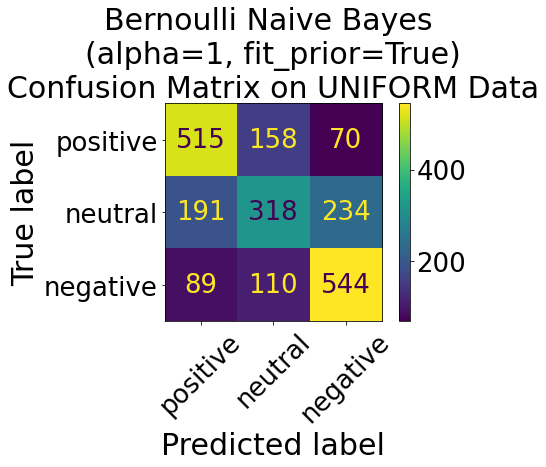
\includegraphics[width = 0.4\textwidth]{cf/BernoulliNaiveBayesalpha1fit_priorTrue-Uniform-confusion-matrix.png}
% 	\caption{Classifier 1's confusion matrix for uniform training and uniform testing data}
% 	\label{fig:cf-1st-uu}
% \end{figure} 

% \begin{figure}[H]
% 	\centering
% 	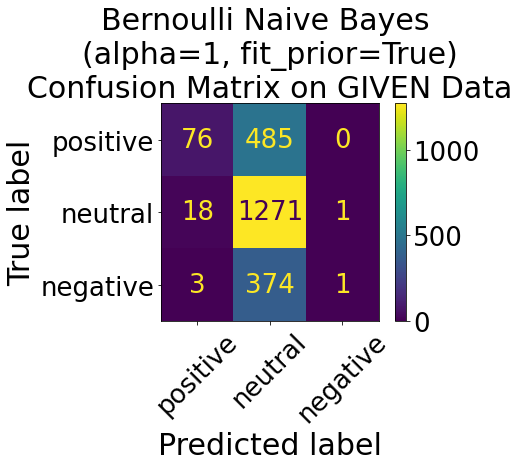
\includegraphics[width = 0.4\textwidth]{cf/BernoulliNaiveBayesalpha1fit_priorTrue-Given-confusion-matrix.png}
% 	\caption{Classifier 1's confusion matrix for given training and given testing data}
% 	\label{fig:cf-1st-rr}
% \end{figure} 

% \begin{figure}[H]
% 	\centering
% 	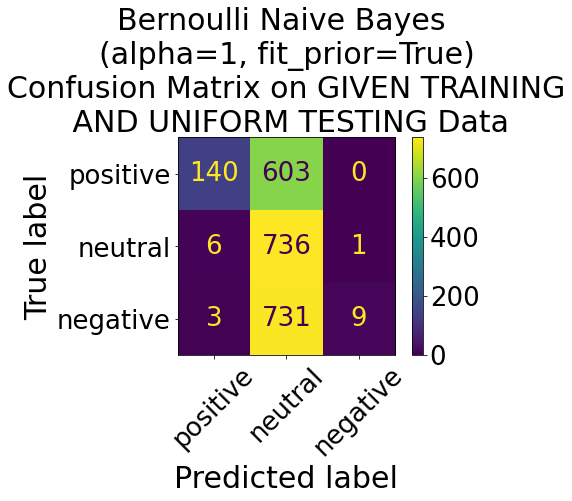
\includegraphics[width = 0.4\textwidth]{cf/BernoulliNaiveBayesalpha1fit_priorTrue-GivenTrainingandUniformTesting-confusion-matrix.png}
% 	\caption{Classifier 1's confusion matrix for given training and uniform testing data}
% 	\label{fig:cf-1st-ru}
% \end{figure} 

% \begin{figure}[H]
% 	\centering
% 	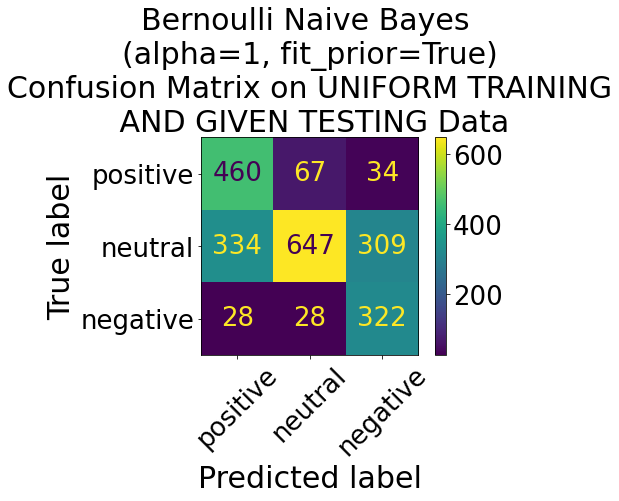
\includegraphics[width = 0.4\textwidth]{cf/BernoulliNaiveBayesalpha1fit_priorTrue-UniformTrainingandGivenTesting-confusion-matrix.png}
% 	\caption{Classifier 1's confusion matrix for uniform training and given testing data}
% 	\label{fig:cf-1st-ur}
% \end{figure} 

% \subsection{Results for Classifier 2}\label{sec:appc2}

\begin{table}[H]
	\begin{center}
		\begin{tabular}{|l|l|}			
			\hline
			Parameter & Value \\
			\hline
			Classifier & Bernoulli N.B. \\
			Include Priors & No \\
			$\alpha$ Smoothing & 1 \\
			\hline\hline
			Uniform Training & Uniform Testing \\
			\hline
			Accuracy & 0.62 \\
			Precisions (+, n, --) 	& 0.65, 0.55, 0.65 \\
			Recalls (+, n, --) 		& 0.70, 0.44, 0.74 \\
			$F_1$ Scores (+, n, --) & 0.67, 0.49, 0.69 \\
			\hline\hline
			Given Training & Given Testing \\
			\hline
			Accuracy & 0.61 \\
			Precisions (+, n, --) 	& 0.73, 0.60, 0.60 \\
			Recalls (+, n, --) 		& 0.16, 0.98, 0.01 \\
			$F_1$ Scores (+, n, --) & 0.26, 0.74, 0.02 \\
			\hline\hline
			Given Training & Uniform Testing \\
			\hline
			Accuracy & 0.42 \\
			Precisions (+, n, --) 	& 0.93, 0.36, 0.95 \\
			Recalls (+, n, --) 		& 0.23, 0.99, 0.03 \\
			$F_1$ Scores (+, n, --) & 0.37, 0.53, 0.05 \\
			\hline\hline
			Uniform Training & Given Testing \\
			\hline
			Accuracy & 0.64 \\
			Precisions (+, n, --) 	& 0.56, 0.87, 0.48 \\
			Recalls (+, n, --) 		& 0.82, 0.50, 0.85 \\
			$F_1$ Scores (+, n, --) & 0.67, 0.64, 0.62 \\
			\hline
		\end{tabular}
		\caption{Classifer 2 metrics}
		\label{tbl:metrics-2nd10000}
	\end{center}
\end{table}

% \begin{figure}[H]
% 	\centering
% 	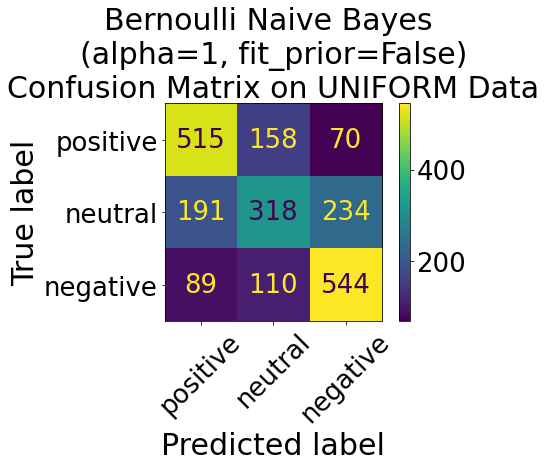
\includegraphics[width = 0.4\textwidth]{cf/BernoulliNaiveBayesalpha1fit_priorFalse-Uniform-confusion-matrix.png}
% 	\caption{Classifier 2's confusion matrix for uniform training and uniform testing data}
% 	\label{fig:cf-2nd-uu}
% \end{figure} 

% \begin{figure}[H]
% 	\centering
% 	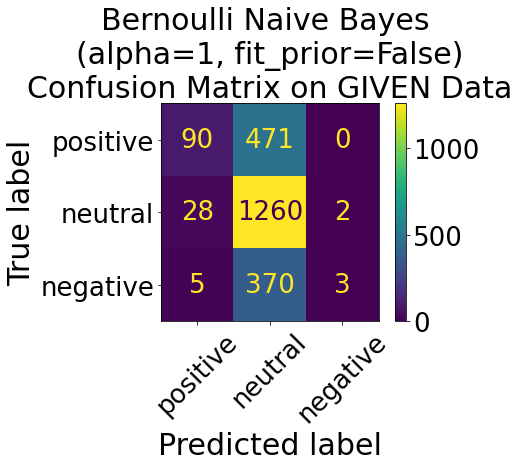
\includegraphics[width = 0.4\textwidth]{cf/BernoulliNaiveBayesalpha1fit_priorFalse-Given-confusion-matrix.png}
% 	\caption{Classifier 2's confusion matrix for given training and given testing data}
% 	\label{fig:cf-2nd-rr}
% \end{figure} 

% \begin{figure}[H]
% 	\centering
% 	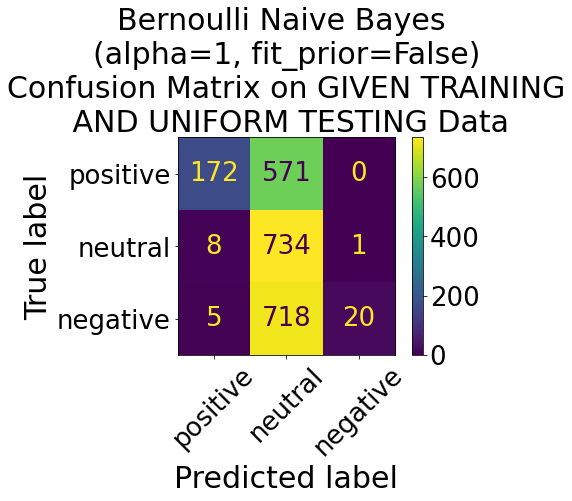
\includegraphics[width = 0.4\textwidth]{cf/BernoulliNaiveBayesalpha1fit_priorFalse-GivenTrainingandUniformTesting-confusion-matrix.png}
% 	\caption{Classifier 2's confusion matrix for given training and uniform testing data}
% 	\label{fig:cf-2nd-ru}
% \end{figure} 

% \begin{figure}[H]
% 	\centering
% 	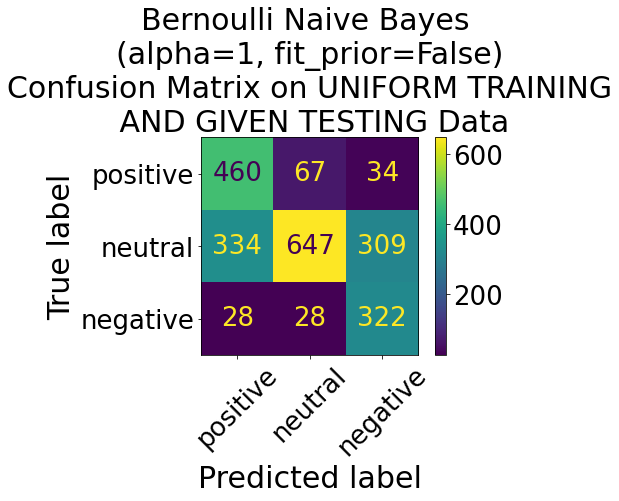
\includegraphics[width = 0.4\textwidth]{cf/BernoulliNaiveBayesalpha1fit_priorFalse-UniformTrainingandGivenTesting-confusion-matrix.png}
% 	\caption{Classifier 2's confusion matrix for uniform training and given testing data}
% 	\label{fig:cf-2nd-ur}
% \end{figure} 

% \subsection{Results for Classifier 3}\label{sec:appc3}

\begin{table}[H]
	\begin{center}
		\begin{tabular}{|l|l|}			
			\hline
			Parameter & Value \\
			\hline
			Classifier & Multinomial N.B. \\
			Include Priors & Yes \\
			$\alpha$ Smoothing & 1 \\
			\hline\hline
			Uniform Training & Uniform Testing \\
			\hline
			Accuracy & 0.62 \\
			Precisions (+, n, --) 	& 0.67, 0.55, 0.62 \\
			Recalls (+, n, --) 		& 0.67, 0.41, 0.78 \\
			$F_1$ Scores (+, n, --) & 0.67, 0.47, 0.69 \\
			\hline\hline
			Given Training & Given Testing \\
			\hline
			Accuracy & 0.61 \\
			Precisions (+, n, --) 	& 0.79, 0.60, 0.20 \\
			Recalls (+, n, --) 		& 0.17, 0.98, 0.00 \\
			$F_1$ Scores (+, n, --) & 0.28, 0.74, 0.01 \\
			\hline\hline
			Given Training & Uniform Testing \\
			\hline
			Accuracy & 0.42 \\
			Precisions (+, n, --) 	& 0.94, 0.36, 1.00 \\
			Recalls (+, n, --) 		& 0.26, 0.99, 0.02 \\
			$F_1$ Scores (+, n, --) & 0.41, 0.53, 0.04 \\
			\hline\hline
			Uniform Training & Given Testing \\
			\hline
			Accuracy & 0.63 \\
			Precisions (+, n, --) 	& 0.58, 0.88, 0.45 \\
			Recalls (+, n, --) 		& 0.79, 0.48, 0.89 \\
			$F_1$ Scores (+, n, --) & 0.67, 0.62, 0.60 \\
			\hline
		\end{tabular}
		\caption{Classifer 3 metrics}
		\label{tbl:metrics-3rd10000}
	\end{center}
\end{table}

% \begin{figure}[H]
% 	\centering
% 	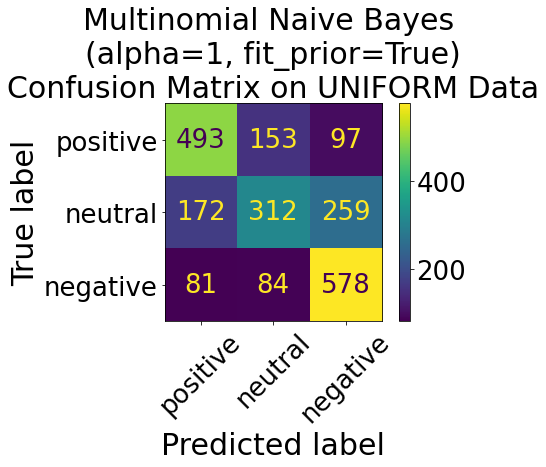
\includegraphics[width = 0.4\textwidth]{cf/MultinomialNaiveBayesalpha1fit_priorTrue-Uniform-confusion-matrix.png}
% 	\caption{Classifier 3's confusion matrix for uniform training and uniform testing data}
% 	\label{fig:cf-3rd-uu}
% \end{figure} 

% \begin{figure}[H]
% 	\centering
% 	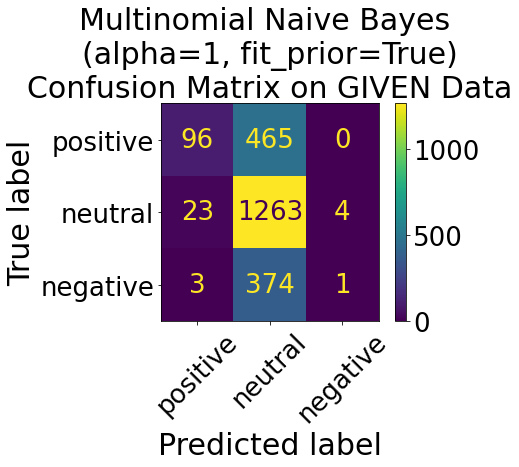
\includegraphics[width = 0.4\textwidth]{cf/MultinomialNaiveBayesalpha1fit_priorTrue-Given-confusion-matrix.png}
% 	\caption{Classifier 3's confusion matrix for given training and given testing data}
% 	\label{fig:cf-3rd-rr}
% \end{figure} 

% \begin{figure}[H]
% 	\centering
% 	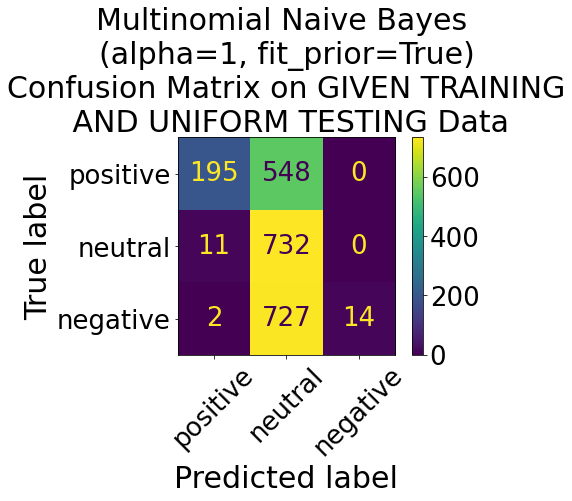
\includegraphics[width = 0.4\textwidth]{cf/MultinomialNaiveBayesalpha1fit_priorTrue-GivenTrainingandUniformTesting-confusion-matrix.png}
% 	\caption{Classifier 3's confusion matrix for given training and uniform testing data}
% 	\label{fig:cf-3rd-ru}
% \end{figure} 

% \begin{figure}[H]
% 	\centering
% 	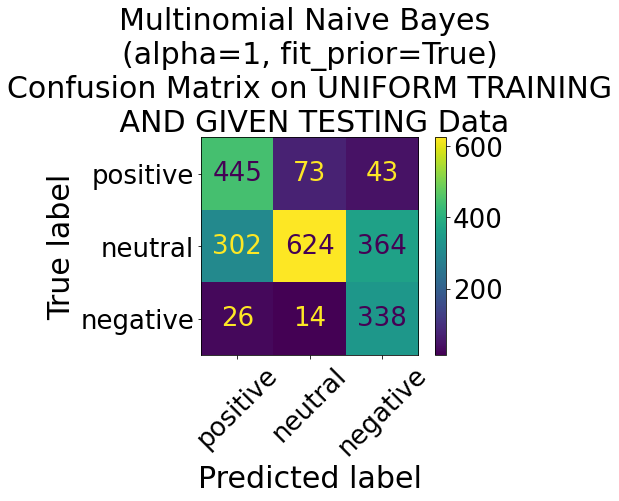
\includegraphics[width = 0.4\textwidth]{cf/MultinomialNaiveBayesalpha1fit_priorTrue-UniformTrainingandGivenTesting-confusion-matrix.png}
% 	\caption{Classifier 3's confusion matrix for uniform training and given testing data}
% 	\label{fig:cf-3rd-ur}
% \end{figure} 

% \subsection{Results for the baseline model (Classifier 4)}\label{sec:appc4}

\begin{table}[H]
	\begin{center}
		\begin{tabular}{|l|l|}			
			\hline
			Parameter & Value \\
			\hline
			Classifier & 0-R \\
			\hline\hline
			Uniform Training & Uniform Testing \\
			\hline
			Accuracy & 0.33 \\
			Precisions (+, n, --) 	& 0.00, 0.00, 0.33 \\
			Recalls (+, n, --) 		& 0.00, 0.00, 1.00 \\
			$F_1$ Scores (+, n, --) & 0.00, 0.00, 0.50 \\
			\hline\hline
			Given Training & Given Testing \\
			\hline
			Accuracy & 0.58 \\
			Precisions (+, n, --) 	& 0.00, 0.58, 0.00 \\
			Recalls (+, n, --) 		& 0.00, 1.00, 0.00 \\
			$F_1$ Scores (+, n, --) & 0.00, 0.73, 0.00 \\
			\hline\hline
			Given Training & Uniform Testing \\
			\hline
			Accuracy & 0.33 \\
			Precisions (+, n, --) 	& 0.00, 0.33, 0.00 \\
			Recalls (+, n, --) 		& 0.00, 1.00, 0.00 \\
			$F_1$ Scores (+, n, --) & 0.00, 0.50, 0.00 \\
			\hline\hline
			Uniform Training & Given Testing \\
			\hline
			Accuracy & 0.17 \\
			Precisions (+, n, --) 	& 0.00, 0.00, 0.17 \\
			Recalls (+, n, --) 		& 0.00, 0.00, 1.00 \\
			$F_1$ Scores (+, n, --) & 0.00, 0.00, 0.29 \\
			\hline
		\end{tabular}
		\caption{Baseline classifier metrics}
		\label{tbl:metrics-base10000}
	\end{center}
\end{table}

% \begin{figure}[H]
% 	\centering
% 	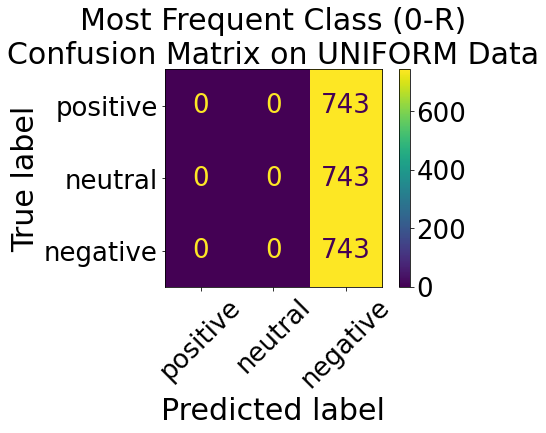
\includegraphics[width = 0.4\textwidth]{cf/MostFrequentClass0R-Uniform-confusion-matrix.png}
% 	\caption{Baseline classifier's confusion matrix for uniform training and uniform testing data}
% 	\label{fig:cf-base-uu}
% \end{figure} 

% \begin{figure}[H]
% 	\centering
% 	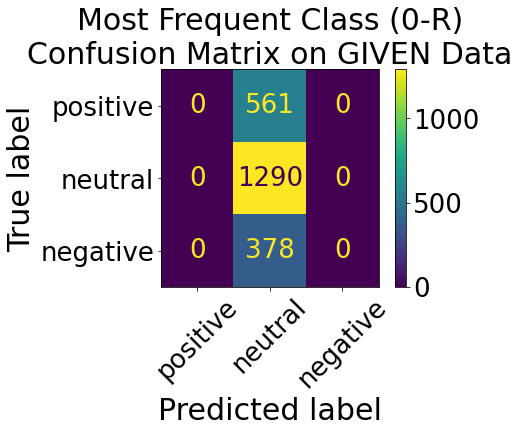
\includegraphics[width = 0.4\textwidth]{cf/MostFrequentClass0R-Given-confusion-matrix.png}
% 	\caption{Baseline classifier's confusion matrix for given training and given testing data}
% 	\label{fig:cf-base-rr}
% \end{figure} 

% \begin{figure}[H]
% 	\centering
% 	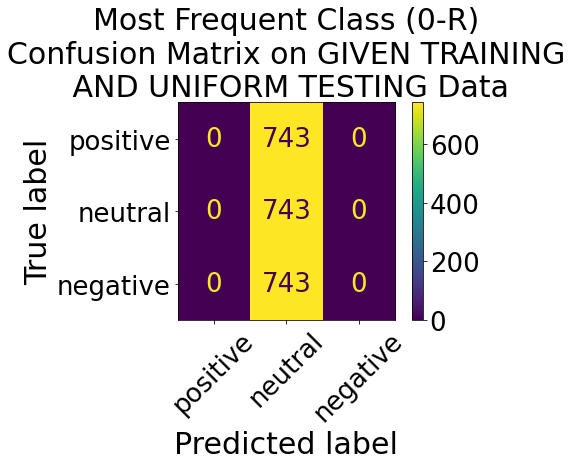
\includegraphics[width = 0.4\textwidth]{cf/MostFrequentClass0R-GivenTrainingandUniformTesting-confusion-matrix.png}
% 	\caption{Baseline classifier's confusion matrix for given training and uniform testing data}
% 	\label{fig:cf-base-ru}
% \end{figure} 

% \begin{figure}[H]
% 	\centering
% 	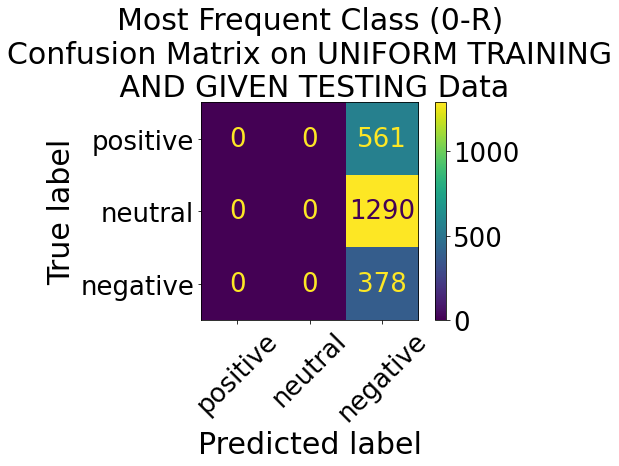
\includegraphics[width = 0.4\textwidth]{cf/MostFrequentClass0R-UniformTrainingandGivenTesting-confusion-matrix.png}
% 	\caption{Baseline classifier's confusion matrix for uniform training and given testing data}
% 	\label{fig:cf-base-ur}
% \end{figure} 

\end{document}
